\subsection{Парадигмы обучения нейронных сетей}

\subsubsection{Обучение с учителем}

Рассмотрим парадигмы обучения нейронных сетей.
Начнем с парадигмы обучения с учителем.

\begin{figure}[h]
\center{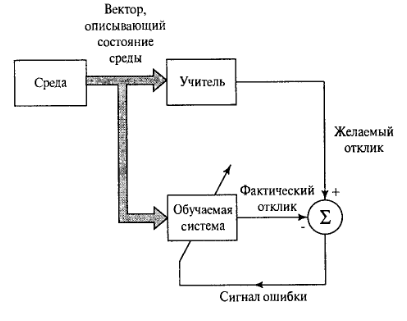
\includegraphics[width=0.6\linewidth]{WithTeacher.png}}
\caption{Блочная диаграмма обучения с учителем}
\label{ris:WithTeacher}
\end{figure}

На рис.~\ref{ris:WithTeacher} приведена блочная диаграмма, иллюстрирующая эту форму обучения. 
Концептуально участие учителя можно рассматривать как наличие знаний об окружающей среде, представленных в виде пар вход-выход.
При этом сама среда неизвестна обучаемой нейронной сети.
Теперь предположим, что учителю и обучаемой сети подается из окружающей среды вектор.
На основе встроенных знаний учитель может сформировать и передать обучаемой нейронной сети желаемый отклик, соответствующий входному вектору.
Этот желаемый результат представляет оптимальные действия, которые должна выполнить нейронная сеть.
Параметры сети корректируются с учетом обучающего вектора и сигнала ошибки.
Корректировка параметров должна выполняться пошагово с целью имитации нейронной сетью поведения учителя.
Эта эмуляция в некотором статистическом смысле должна быть оптимальной.
Таким образом, в процессе обучения знания учителя передаются в сеть в максимально полном объеме.

\subsubsection{Обучение без учителя}

Обучение без учителя осуществляется без вмешательства внешнего учителя или корректора, контролирующего процесс обучения.
Существует лишь независимая мера качества представления, которому должна научиться нейронная сеть, и свободные параметры сети оптимизируются по отношению к этой мере.
После обучения сети на статистические закономерности входного сигнала она способна формировать внутреннее представление кодируемых признаков входных данных, и таким образом, автоматически создавать новые классы.

Для обучения без учителя можно воспользоваться правилом конкурентного обучения.
Например, можно использовать нейронную сеть, состоящую из двух слоев --- входного и выходного.
Входной слой получает доступные данные.
Выходной слой состоит из нейронов, конкурирующих друг с другом за право отклика на признаки, содержащиеся во входных данных.
В простейшем случае нейронная сеть действует по принципу <<победитель забирает всё>>.
При этом все остальные нейроны отключаются.